\documentclass[11pt, a4paper]{article}
\usepackage{natbib}
\usepackage{eso-pic}
\usepackage{amsmath} % flere matematikkommandoer
\usepackage{amssymb}
\usepackage[utf8]{inputenc} % æøå
\usepackage[T1]{fontenc} % mere æøå
\usepackage[danish, english]{babel} % orddeling
\usepackage{verbatim} % så man kan skrive ren tekst
\usepackage{graphicx}
\usepackage{booktabs}
\usepackage{enumitem}
\usepackage{placeins}
\usepackage[colorlinks=false]{hyperref}
\usepackage{tocbibind}

\author{
    Christian Kjær Larsen \texttt{(011292)} \\[.4cm]
    Lukas Svarre Engedal \texttt{(210790)} \\[.4cm]
    Tobias Sønderskov Hansen \texttt{(240395)} \\[.4cm]
    Instruktor: Aske Mottelson\\[.4cm]
    \vspace{9cm}
}

\title{
  \vspace{3cm}
  \Huge{PoP-Webhelp} \\[.10cm]
  \Large{Delrapport 2, ProjDat 2015}
}

\begin{document}
\selectlanguage{danish}
\AddToShipoutPicture*{\put(0,0){\includegraphics*[viewport=0 0 700 600]{includes/nat-farve}}}
\AddToShipoutPicture*{\put(0,602){\includegraphics*[viewport=0 600 700 1600]{includes/nat-farve}}}

%% Change `ku-en` to `nat-en` to use the `Faculty of Science` header
\AddToShipoutPicture*{\put(0,0){\includegraphics*{includes/nat-en}}}

\clearpage\maketitle
\thispagestyle{empty}

\newpage

\selectlanguage{english}
\begin{abstract}
    This report presents the development of an e-learning system for use in the newly created introductory computer science course at the Institute of Computer Science at the University of Copenhagen, called \emph{Programmering og Problemløsning}. Our clients are Martin Dybdal and Oleksandr Shturmov, both employed at the institute, who will be in charge of the course. In the course, the students will be taught the programming language \verb!F#!.

    The aim of the e-learning system is to introduce new students to programming in a simple and user-friendly way, and to teach them various basic ideas and concepts in programming in general, and \verb!F#! in particular. This is done by presenting the students with an array of different exercises, sorted based on subject and difficulty, and presented to students in a specific and meaningful order.

The system will have two different kinds of users: students and admins.

Students will mainly be working on the various exercises, and they will also be able to get hints for the exercises if needed and provide feedback on the exercises and hints once completed. Students should also be able to see how well they are doing so far, for instance how many of the exercises belonging to a particular subject matter they have solved.

The primary role of the admins will be managing the exercises and supervising how well the students are doing. They should be able to easily delete or modify existing exercises or add new ones, as well as manage the order in which the students are presented with the exercises. They should also be able to get various statistics about how the students are doing in order to improve and optimize the exercises, their order and their subjects.
\end{abstract}
\newpage
\tableofcontents

\thispagestyle{empty}

\newpage
\pagestyle{plain}
\setcounter{page}{1}
\pagenumbering{arabic}

\selectlanguage{danish}
\section{Review}
\subsection{Designing for usability: key principles and what designers think}
\label{sub:designing_for_usability}
\paragraph{Referat}
Gould og Lewis\cite{gould1985designing} beskriver en overordnet metode til design og udvikling af brugervenlige systemer. Denne tilgangsvinkel består af tre grundlæggende principper: tidligt fokus på brugerne, empiriske målinger og iterativt design. Artiklen tager udgangspunkt i udviklingen af IBM's \emph{Audio Distribution System} (ADS) hvor disse principper blev anvendt.

Ved første princip påstås at det er nødvendigt for systemudviklerne fra starten at sætte sig ind i hvem systemets tiltænkte målgruppe er. Metoden anbefaler at udviklerne danner sig en \emph{forståelse} for brugerne, frem for blot at lave en karakterisering. Udover selve brugerne, skal udviklerne også sætte sig ind i hvilken sammenhæng systemet skal bruges og hvilke opgaver det skal løse, samt hvordan et evt. nuværende system løser disse opgaver.

Andet princip, \emph{empiriske målinger}, beskriver brugen af prototyper og simulering til at teste mod målgruppen for at studere dennes reaktion. Personer der selv har været med til at udvikle systemet vil næsten uundgåeligt anvende systemet anderledes end en typisk bruger, derfor er det vigtigt at systemet også bliver afprøvet af målgruppen, og at målgruppens respons bruges i den efterfølgende udvikling.

\emph{Iterativt design} går ud på at de problemer der opdages under afprøvningen skal løses. Dette sikres ved at opdele systemudviklingen i en masse gentagelser af design og afprøvning, hvor resultaterne af afprøvningen i én iteration påvirker deisgnet i den næste. Dette er i kontrast til mere lineære modeller, hvor der i stedet udarbejdes en detaljeret kravspecifikation, og en egentlig afprøvning først sker til sidst i projektet.

Når udviklere præsenteres for disse principper er reaktionen typisk at det virker meget intuitivt og mange påstår at de allerede anvender disse principper. Ifølge undersøgelser foretaget af folkene bag metoden tyder det dog på, at der er forskel på hvad systemudviklerne selv siger de gør, og hvad de egentlig gør i praksis.

\paragraph{Perspektivering}
De tre principper fra artiklen indgår alle i et vist omfang i systemudviklingsmetoden præsenteret i OOSE.

Med hensyn til tidligt fokus på brugerne, så inkorporerer OOSE's fremgangsmåde bl.a. dette i form af en \emph{requirements elicitation}, der beskriver de forskelllige typer brugere og i hvilke sammenhænge de systemet anvendes.

Artiklen understreger vigtigheden af at kunne foretage ændringer baseret på brugernes reaktioner, derfor er det vigtigt at systemet er struktureret på en måde der tager højde for dette. Man kan sammenligne dette med \emph{Entity-Boundary-Control} fremgangsmåden beskrevet i OOSE \cite{OOSE}, der fokuserer på at opdele systemet i nogle forholdsvis uafhængige elementer, så der eksempelvis kan ændres i brugergrænsefladen uden at det påvirker resten af programmet.

Både metoden beskrevet i artiklen og de fremgangsmåder præsenteret i OOSE er agile. Den grundlæggende metode er altså fælles for dem alle, udviklingen sker i iterationer af henholdsvis design og brugertest.

\subsection{A Rational Design Process: How and Why to Fake It}
\label{sub:a_rational_design_process}
\paragraph{Referat}
Parnas og Clements \cite{parnas1986rational} prøver i artiklen at beskrive en ideel udviklingsproces og den dokumentation der kræves. Hovedargumentet i artiklen er dog, at selvom man ikke har fuldt grundlag for en altomfattende kravspecifikation, så skal man stadig producere dokumentation som hvis man havde.

Derfor mener forfatterne, at hvis man ikke har en helt beskrivende kravspecifikation, så er det vigtigt at kende processen, så man som udvikler kan hjælpe designerne med, at finde de manglende informationer. Det gør, at man tidligere i processen kan få fundet fejl i designet, så de ikke kommer med i det endelige system.

Den metode som Parnas og Clements foreslår i artiklen er, at man starter med at dokumentere krav. Dette er med til at gøre det lettere at estimere tidsforbruget, blive klog på problemområdet for alle involverede og hjælpe med ting som test, inkonsistens og udskiftning af personer, da den specifikke viden er skrevet ned.

Derefter mener de, at man skal nebryde arbejdet i moduler, så det kan uddelegeres til forskellige udviklere. Grænsefladerne mellem modulerne og selve kravene til modulerne dokumenteres grundigt. Til sidst produceres kildekoden, og produktet er klart. Der argumenteres for, at hvis alt forarbejdet er gjort grundigt, så er programmeringen ligetil.

Hele titlen på artiklen, det at \emph{fake} den ideelle udviklingsproces går ud på, at hvis man følger den ideelle proces, så når man mangler et stykke information, så noterer man dette i designdokumentationen. Når man så finder de rigtige svar senere, så rettes dokumentationen hele vejen ned i kæden. Dette skulle så meget gerne producere en korrekt specifikation i sidste ende.

\paragraph{Perspektivering}
Den idealiserede udviklingsproces som beskrives i \cite{parnas1986rational} har mange ting til fælles med nogle af kapitlerne i \cite{OOSE}. Den i artiklen omtalte kravspecifikation har mange ting til fælles med det i bogen omtalte \emph{Requirement Analysis Document} (Kapitel 4). I begge dokumenter indgår alle informationer, der skal til at udvilkle systemet.

I artiklen beskrives hvordan dette dokument kan bruges til at nedbryde problemet i moduler som kan takles af mange forskellige udviklere. Det er også hvad der foreslås i kapitel 6 i \cite{OOSE}. Her nedbrydes systemet efter analysemodellen som er resultatet af kravspecifikationen. Det er også her, ligesom i artiklen, at grænsefladerne mellem modulerne specificeres, så en udvikler nemt og fejlfrit kan udvikle delsystemet. I artiklen argumenterer forfatterne for, at for hvert delsystem, så skal der fremstilles en kravspecifikation med samme struktur som for hele systemet. Det bliver en slags rekursiv dokumentation, da et delsystem godt kan bestå af flere. Fra et ledelsesperspektiv er det beskrevet i kapitel 14 i \cite{OOSE} hvordan denne nedbrydning uddelegeres mellem udviklere, så arbejdet foregår mest effektivt.

Artiklen omtaler processen som ideel. Den omtalte proces er i praksis det vi kender som \emph{vandfaldsmodellen}. I mere moderne softwareudvikling stiller man spørgsmålstegn ved, om det er den optimale proces. Det er især efter udbredelsen af agile metoder som \emph{SCRUM} \cite{sutherland2010jeff} og andre. Her erkender man, at det er nærmest umuligt at designe software på samme måde som man designer broer på, da der simpelthen er for mange ukendte faktorer når man starter. Dette udbedres så ved at beskrive kravene samtidig med at systemet udviklet, da det så er nemmere at finde fejl i designet undervejs.

\newpage
\section{Formål og rammer}
\label{sec:formal_og_rammer}
I dette afsnit beskrives systemets formål og rammer ved \textit{FACTOR}-kriteriet.
\paragraph{Funktionalitet}
\begin{itemize}
    \item Besvare programmeringsspørgsmål
    \item Oprette programmeringsspørgsmpl
    \item Analysere det studerendes fremskridt
    \item Håndtere de studerendes login
\end{itemize}
\paragraph{Anvendelsesområde}
\begin{itemize}
    \item Undervisere ved DIKU
    \item Førsteårsstuderende ved DIKU
\end{itemize}
\paragraph{Betingelser}
\begin{itemize}
    \item Undervisere har begrænsede resurser
    \item Det skal foregå online
\end{itemize}
\paragraph{Teknologi}
\begin{itemize}
    \item Python 2
    \item Flask webframework
    \item SQLAlchemy
    \item HTML/CSS
    \item Javascript
\end{itemize}
\paragraph{Objekter}
Studerende, Spørgsmål, Hint, Underviser.
\paragraph{Ansvar}
E-læringssystem der skal hjælpe de studerende med programmering.

\section{Kravspecifikation}
\label{sec:kravspecifikation}
I dette afsnit beskrives kravene til systemet. Det er ting som de funktionelle og de ikke-funktionelle krav til systemet. Der er også diagrammer der uddybber systemets funktionalitet og udformning.
\subsection{Krav}
\label{sub:krav}
\paragraph{Funktionelle krav}
De funktionelle krav for systemet er i tråd med afsnit 4.3.1 i \cite{OOSE}, nemlig at de omhandler den specifikke brug af systemet.
\begin{itemize}
    \item Systemet skal være en hjemmeside med opgaver, som kan løses individuelt af studerende.
    \item Der kræves login, så man kan følge med i den studerendes udvikling.
    \item Spørgsmålene skal være grupperede efter hvilke læringsmål de tester.
    \item Læringsmålene skal igen grupperes i nogle blokke, hvor idéen så er at man gennemgår blokkene én af gangen i en bestemt rækkefølge, og at sværhedsgraden stiger løbende.
    \item Der skal være hints til opgaverne som de studerende kan benytte hvis nødvendigt, og de studerende skal så kunne give feedback til hints'ne.
    \item Alle forsøg på opgavebesvarelser skal gemmes i en log.
\end{itemize}
Hvis der er tid i en af de senere iterationer, så er der en række ekstra krav som kan implementeres.
\begin{itemize}
    \item Loggen skal bruges til at give underviseren information om hvilke spørgsmål der er svære.
    \item Der skal tilføjes en grad af \emph{gamification}, så der gives badges og point for fremskridt, og det bliver muligt at følge med i andres fremskridt.
    \item Hvis man ikke har øvet sig i et emne i et stykke tid, så falder ens erfaring i området.
\end{itemize}

\paragraph{Ikke-funktionelle krav}
\label{par:ikke_funktionelle_krav}
I afsnit 4.3.2 i \cite{OOSE} beskrives ikke-funktionelle krav som krav, der ikke direkte beskriver funktionaliteten, men mere generelle krav omkring ting som brugervenlighed, ydeevne, pålidelighed og hvor vedligeholdesesvenligt systemet er.

De ikke-funktionelle krav til dette projekt er forholdsvis begrænsede, idet vi har fået ret stor frihed i forhold til hvordan vi løser opgaven af vores kunde.

\begin{itemize}
\item Det skal være nemt at tilføje nye opgaver til systemet, sådan at kursuslederne efterfølgende kan opbygge en tilstrækkelig samling af opgaver til de studerende.
\item Det endelige produkt skal gerne skal være simpelt og modulært, sådan at det er nemt at overtage, udvide og bygge videre på efter at vi overgiver projektet til kunden.
\item Ingen af kunderne er web-udviklere, så det er også vigtigt at det valgte framework er veldokumenteret og rimeligt simpelt at bruge.
\end{itemize}

\subsection{Use case model}
\label{sub:use_case_model}
På Figur \ref{fig:use_case_model} kan man se vores use case model diagram. Vi har at gøre med to aktører, nemlig studerende og administratorer. Det vigtige for studerende er at de kan oprette sig på siden, og at de har adgang til opgaver de kan besvare. Det vigtige for administratorer er at de kan administrere opgaverne, og at de kan få feedback og statistik på hvordan de studerende klarer opgaverne. Begge aktører skal desuden kunne benytte simpel funktionalitet i forbindelse med deres login.
\begin{figure}[h]
  \centering
  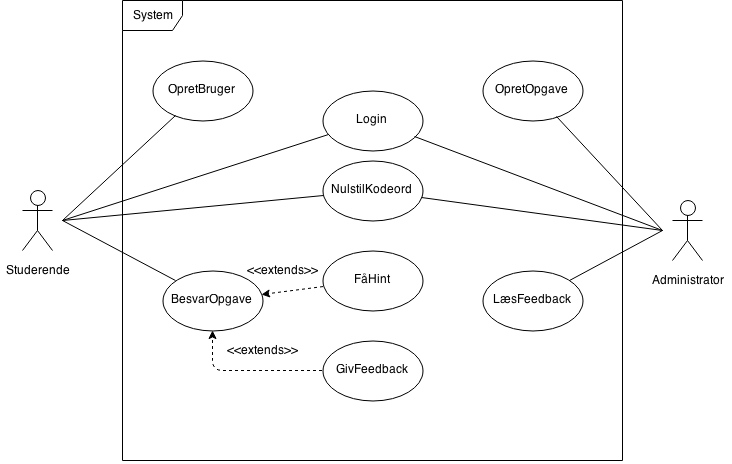
\includegraphics[width=0.8\linewidth]{figures/UseCaseModel.png}
  \caption{Use case model for vores system.}
  \label{fig:use_case_model}
\end{figure}
\subsection{Use cases}
\label{sub:use_cases}

På Figur \ref{fig:use_case1} ses en beskrivelse af use casen, hvor en studerende opretter sin bruger. Det er en simpel use case, der beskriver i detaljer hvordan processen med at oprette sig som bruger i systemet skal foregå. Inden denne use case, så har brugeren ikke oprettet sig, og når use casen er fuldført, så har brugeren oprettet sig, er godkendt og logget ind. Det kombinerer en del af funktionaliteten i én use case. Det kunne godt deles op, men da vi her kun skal beskrive tre overordnede use cases, så har vi kombineret dem.
\begin{figure}[h!]
    \centering
    \begin{tabular}{r p{8cm}}
        \toprule
        \textit{Navn på use-case:} & \verb!OpretBruger! \\
        \hline
        \textit{Deltagende aktører:} & Påbegyndt af en studerende \\
        \hline
        \textit{Hændelser:} & \begin{enumerate}[nolistsep]
            \item En studerende åbner hjemmesiden og klikker på \verb!register!
            \item Den studerende indtaster sine brugeroplysninger, dvs. ku-id og løsen.
            \item Systemet opretter brugeren, og sender en e-mail med et aktiveringslink.
            \item Den studerende klikker på linket, og kontoen aktiveres.
            \item Den studerende bringes til login-siden.
            \item Den studerende indtaster ku-id og løsen og klikker \verb!Login!
            \item Der informeres om succesfuldt login, og brugeren bringes til applikationen.
        \end{enumerate}  \\
        \hline
        \textit{Startbetingelse:} & En studerende har ingen konto, og er ikke logget ind. \\
        \hline
        \textit{Slutbetingelse:} & En studerende har en aktiveret konto og er logget ind. \\
        \bottomrule
    \end{tabular}
    \caption{Use case omkring oprettelse af brugere.}
    \label{fig:use_case1}
\end{figure}

På Figur \ref{fig:use_case2} ses en beskrivelse af use casen, hvor en studerende svarer på spørgsmål. Den er på et relativt højt abstraktionsniveau, da vi ikke er helt sikre på hvordan workflowet i systemet er endnu. En ting er dog sikkert. Når man har valgt et emne, så vil der blive stillet spørgsmål i en lind strøm, indtil systemet finder at man har dygtiggjort sig nok inden for emnet til at man kan begynde på et nyt.
\begin{figure}[h!]
    \centering
    \begin{tabular}{r p{8cm}}
        \toprule
        \textit{Navn på use-case:} & \verb!BesvarOpgave! \\
        \hline
        \textit{Deltagende aktører:} & Påbegyndt af en studerende \\
        \hline
        \textit{Hændelser:} & \begin{enumerate}[nolistsep]
            \item En studerende åbner hjemmesiden.
            \item Vedkommende vælger et emne inden for en læringsblok der er låst op ved at have færdiggjort den forrige.
            \item Systemet præsenterer et spørgsmål for den studerende. Der kan være flere typer spørgsmål (multiple-choice, udfyldning med flere).
            \item Den studerende indtaster et svar.
            \item Systemet giver respons på svaret, og gemmer det i en historik.
            \item Den studerende trykker næste, for at få et spørgsmål mere.
            \item Hvis den studerende har svaret på nok spørgsmål, så kan den studerende vælge en ny kategori.
            \item Den studerende lukker browseren.
        \end{enumerate}  \\
        \hline
        \textit{Startbetingelse:} & En studerende der er logget ind. \\
        \hline
        \textit{Slutbetingelse:} & En studerende der er logget ind og har besvaret en eller flere opgaver. \\
        \bottomrule
    \end{tabular}
    \caption{Use case omkring besvarelse af opgaver.}
    \label{fig:use_case2}
\end{figure}

Et af kravene for systemet er, at det skal være nemt for underviserne i kurset at oprette nye opgaver. Da underviserne selv er dataloger, så vil det være optimalt hvis man kan lave spørgsmålene i et struktureret filformat. Vi har foreslået \verb!YAML!, derfor er use-casen på Figur \ref{fig:use_case3} meget simpel, og består kun af fil-upload.
\begin{figure}[h!]
    \centering
    \begin{tabular}{r p{8cm}}
        \toprule
        \textit{Navn på use-case:} & \verb!OpretOpgave! \\
        \hline
        \textit{Deltagende aktører:} & Påbegyndt af en administrator \\
        \hline
        \textit{Hændelser:} & \begin{enumerate}[nolistsep]
            \item Vedkommende trykker på \verb!Add Question!.
            \item En YAML fil uploades i en formular.
            \item Brugeres informeres om at spørgsmålet er oprettet.
        \end{enumerate}  \\
        \hline
        \textit{Startbetingelse:} & En administrator der er logget ind. \\
        \hline
        \textit{Slutbetingelse:} & En administrator der er logget ind og har oprettet en opgave. \\
        \bottomrule
    \end{tabular}
    \caption{Use case omkring oprettelse af opgaver.}
    \label{fig:use_case3}
\end{figure}

\subsection{Klassediagram}
\begin{figure}[h]
    \centering
    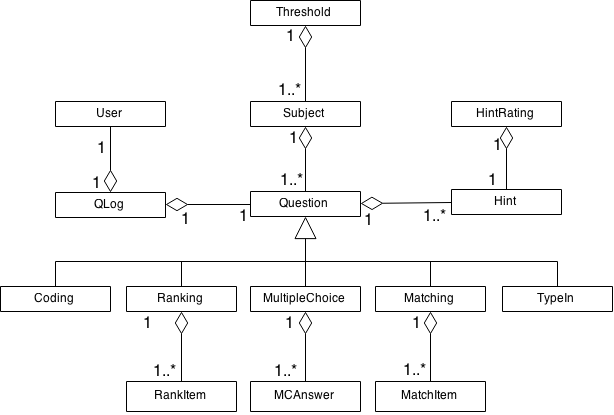
\includegraphics[width=0.8\linewidth]{figures/ClassDiagram.png}
    \caption{Klassediagram af problemområdet}
    \label{fig:class_diagram}
\end{figure}
På Figur \ref{fig:class_diagram} kan man se vores klassediagram. Størstedelen af klasserne har at gøre med opgaverne og deres inddeling i forskellige grupper samt de forskellige typer af opgaver der findes. Derudover er der et par klasser der har at gøre med den log der føres over de studerendes opgavebesvarelser, for at de kursusansvarlige kan følge med i hvad der går godt og mindre godt. Endeligt er der en klasse for studerende og en klasse for administratorne.
\subsection{BCE-model}
\begin{figure}[h]
  \centering
  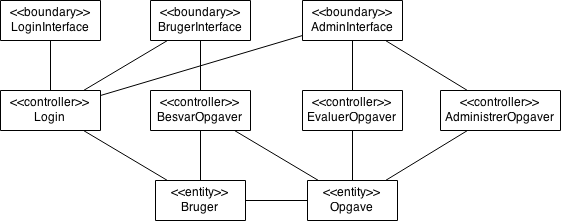
\includegraphics[width=0.8\linewidth]{figures/BCE-Model.png}
  \caption{BCE model for vores system.}
  \label{fig:bce_model}
\end{figure}
På Figur \ref{fig:bce_model} kan man se vores BCE model. Modellen har to entity-objekter, fire controller-objekter samt tre boundary-objekter.

De to entity-objekter er \emph{Bruger} og \emph{Opgave}. \emph{Bruger} indeholder informationer om hver enkelt bruger som login-oplysninger, hvor vidt brugeren er en studerende eller en admin samt hvilke opgaver brugeren allerede har løst. \emph{Opgave} indeholder alle informationerne om de enkelte opgaver, det er både selve opgaven der skal løses samt statistik omkring hvordan det er gået når studerende har løst opgaven.

Modellen har tre boundary-objekter, hvor det første man vil møde når man indlæser siden er \textit{login}-brugergrænsefladen, der sammen med \emph{login}-controlleren sørger for at logge brugerne ind i systemet. Derefter vil man så enten have adgang til \emph{Bruger}-grænsefladen eller \emph{Admin}-grænsefladen afhængig af hvad ens status er, og derfra har man adgang til en række controllers.

Modellen har fire controller-objekter, hvor den første er \emph{login}-controlleren der som tidligere nævnt står for at logge brugere ind i systemet. Som studerende vil man have adgang til \emph{BesvarOpgave}-controlleren, der snakker sammen med \emph{Bruger} og \emph{Opgave} og sørger for at stille brugeren de rigtige opgaver. Som admin vil man have adgang til to controllers, nemlig \emph{EvaluerOpgave}-controlleren og \emph{AdministrerOpgave}-controlleren. \emph{EvaluerOpgave}-controlleren snakker sammen med \emph{Opgave} og giver en adgang til de forskellige slags statistik der bliver samlet om opgaverne, og \emph{AdministrerOpgave}-controlleren snakker ligeledes sammen med \emph{Opgave} og giver en adgang til at slette eller ændre i eksisterende opgaver samt tilføje nye.

\subsection{Sekvens-diagrammer}
I dette afnit er der lavet sekvensdiagrammer over de tre use cases der er beskrevet i Afsnit \ref{sub:use_cases}.
\begin{figure}[h]
    \centering
    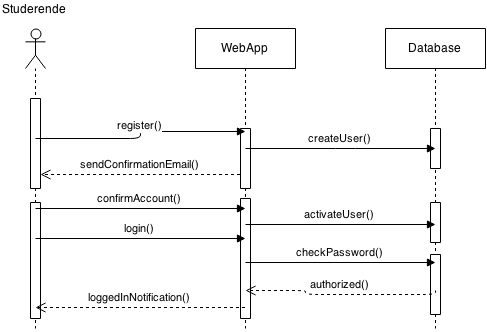
\includegraphics[width=0.8\linewidth]{figures/OpretBrugerUseCase.png}
    \caption{Sekvensdiagram over opretning af bruger}
    \label{fig:opret_bruger_sekvens}
\end{figure}
På Figur \ref{fig:opret_bruger_sekvens} kan man se sekvens-diagrammet for den første use case, der beskriver hvordan en studerende opretter sig som bruger i systemet. Her indgår to adskilte sessioner. En hvor brugeren opretter sig. Så sender systemet en email til brugeren. I næste session klikker brugeren på et link i denne email, og brugeren aktiveres. Derefter logger vedkommende ind. Brugeren gøres opmærksom på at dette er lykkedes, og use casen er færdig.

\begin{figure}[h]
    \centering
    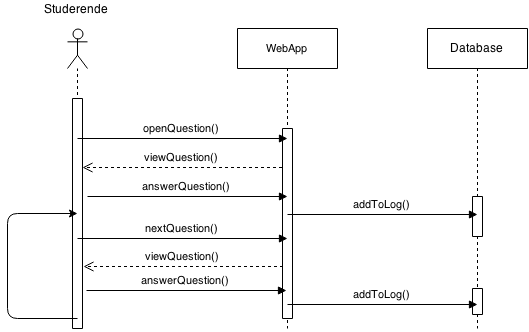
\includegraphics[width=0.8\linewidth]{figures/SvarUseCase.png}
    \caption{Sekvensdiagram over besvarelse af spørgsmål}
    \label{fig:svar_sekvens}
\end{figure}
På Figur \ref{fig:svar_sekvens} kan man se sekvens-diagrammet for den anden use case, der beskriver hvordan en studerende besvarer spørgsmål. Brugeren åbner et spørgsmål, og kan ved at svare kommer videre til næste spørgsmål. Løkken viser at der kan komme flere end et spørgsmål efter det første.

\begin{figure}[h]
    \centering
    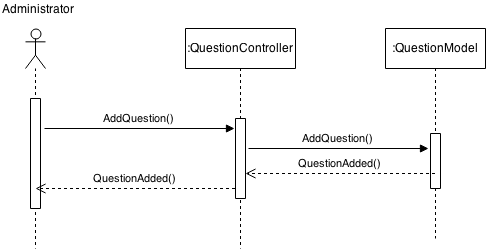
\includegraphics[width=0.8\linewidth]{figures/OpretSporgsmalUseCase.png}
    \caption{Sekvensdiagram over opretning af spørgsmål}
    \label{fig:opret_sp_sekvens}
\end{figure}
På Figur \ref{fig:opret_sp_sekvens} kan man se sekvens-diagrammet for den tredje use case, der beskriver hvordan en administrator opretter et nyt spørgsmål i systemet. Dette sekvensdiagram er stort set linært, da der ikke sker mere ed at der uploades et spørgsmål, og der gives respons på at det er tilføjet korrekt.

\section{Systemdesign}
\label{sec:systemdesign}
I dette afsnit beskrives de designopgaver der er udført allerede. Til sidst i afsnittet vises de dele der endnu ikke er udført.
\subsection{Strukturering}
\label{sub:strukturering}

I nogle udviklingsmiljøer er der typisk givet en struktur af kodebasen på forhånd. Det gælder mange gange når man bruger store frameworks som Django til Python eller Play til Java. Der er nogle konventioner til hvilke klasser der skal i hvilke mapper, og til hvordan konfigurationsfiler skal struktureres. Det er med til at tvinge god strukturing af koden. Frameworket Flask, som vi har valgt at bruge, har ikke sådanne konventioner. Alt kunne placeres i en stor fil hvis det skulle være. Derfor har vi været omhyggelige med at organisere moduler og klasser på en sådan måde at det er nemt at finde hoved og hale i.

Det giver god mening som den første nedbrydning at dele applikationen op i moduler, som hver især indkapsler indkapsler adskildt funktionalitet. Det beskrives også i kapitel 6.3 i \cite{OOSE}, hvor det beskrives hvordan man får delt et system op, så kohæsionen mellem moduler bliver så lille som mulig. Ud fra kravspecifikationen har vi nedbrudt det til følgende moduler:
\begin{description}
    \item[\texttt{admin}] Håndterer opgaver med administration af spørgsmål, kategorier og brugere.
    \item[\texttt{log}] Håndterer opgaver med logning af statistik fra opgaver og visning af denne.
    \item[\texttt{question}] Håndterer opgaver omkring visning og besvarelse af opgaver.
    \item[\texttt{user}] Håndterer brugerlogins, og alt der hører med af oprettelse, ændring af password, nulstilning osv.
\end{description}

Det har gjort at vi har kunnet takle problemer uafhængigt af hinanden, og derved har kunnet udvikle mere effektivt.

\subsection{Databasedesign}
\label{sub:databasedesign}
I Appendix \ref{sec:er_diagrams} ses tre ER-diagrammer der illustrerer opbygningen af vores database. 

På Figur \ref{fig:er_diagram_question} ses den del der har at gøre med spørgsmålene. Det er stort set identisk med klassediagrammet over vores problemområde som ses på Figur \ref{fig:class_diagram}. Her er den generelle struktur over hvordan spørgsmålene er inddelt uddybet. Altså hvordan et \emph{Question} hører til et \emph{Subject}, der igen hører til et \emph{Threshold} og så videre. Vi prøver også at vise den modulære struktur hvor vi har ladet nye typer spørgsmål nedarve fra en generaliseret type.

På Figur \ref{fig:er_diagram_log} ses den del der har med loggen at gøre. Hver gang en studerende vælger et emne og begynder at svare på spørgsmål bliver der oprettet en session, som sørger for at holde styr på hvilke spørgsmål den studerende svarer på i den omgang. Efter hvert spørgsmål den studerende svarer på bliver der desuden logget en masse informationer om dette. Endelig bliver det gemt når en studerende giver en vurdering af et specifikt hint.

Det tredje og sidste ER-diagram kan ses på Figur \ref{fig:er_diagram_user}, og har at gøre med brugere. Her bliver alt informationen om de studerende og deres kontoer gemt, samt informationer om admins.

\subsection{Implementeret funktionalitet}
\label{sub:implementeret_funktionalitet}
Vi har med ER-diagrammet i hånden implementeret en lang række klasser med hjælp fra \verb!SQLAlchemy!, som er en \emph{Object Relational Mapper} til python, der sørger for, at det er nemt at kunne lave python objekter ud fra en række i databasen. Disse klasse dækker over alle de forskellige typer af spørgsmål, samt de forskellige log-elementer.

Oven på det har vi med hjælp fra \verb!Flask! frameworket implementeret en simpel web applikation der har funktionalitet til at håndtere brugerlogins og som kan vise og give respons på spørgsmål og præsentere dem og de \emph{Subjects} og \emph{Thresholds} de hører ind under.

\subsection{Udestående design- og implementationsopgaver}
\label{sub:udestaende_design_og_implementationsopgaver}
De to vigtigste udeståender er implementeringen af hele logningen af data, samt admin aspektet af projektet.


\section{Program- og systemtest}
\label{sec:program_og_systemtest}
I dette afsnit uddybes vores teststrategi, og hvordan testene er forløbet.
\subsection{Unittests}
\label{sub:unittests}
For at det skal være så nemt og smertefrit som muligt at teste, så bruger vi et automatisk unittest værktøj. Ifølge \cite{COCO}, så er automatiske tests den eneste reelle måde at teste på. En af fordelene i vores tilfælde er, at hvis man laver mange ændringer i koden, som der ofte er, når man arbejder agilt, så er det vigtigt at man kan køre testene hurtigt og nemt efter hver ændring af koden. Vi bruger det inkluderede testbibliotek i \verb!Python! nemlig \verb!unittest!\footnote{\url{https://docs.python.org/2/library/unittest.html}}. Det virker på samme måde som \verb!JUnit! i \verb!Java!, hvor man skriver testmetoder i en testklasse.

For at være sikker på at vores tests er dækkende, så bruges et værktøj der måler dækningsgraden (Afsnit 11.4.3 i \cite{OOSE})  af vores tests. Det giver en metrik af hvor gode testene er. Dette værktøj er \verb!coverage!\footnote{\url{http://nedbatchelder.com/code/coverage/}}. Det kan også generere rapporter, som viser et overblik over koden, og visuelt viser hvilke dele af koden der er dækket af tests.

På Figur \ref{fig:testcoverage} ses en udskrift af testrapporten. Der ses hvilke moduler af koden, som er dækket tilstrækkeligt af tests. På Figur \ref{fig:code_coverage} ses hvordan værktøjet viser hvilke dele af koden der er dækket af tests.

\subsection{Integrationstests}
\label{sub:integrationstests}
Når vi har flere færdiggjorte moduler, så skal de testes sammen med realistiske input data, for at se om flere dele af systemet spiller sammen.

\subsection{Usability-tests}
\label{sub:usability_tests}
Når vi har en funktionsdygtig brugergrænseflade, så skal der udføres tests af hvor brugervenlig den er.

\begin{figure}[h]
    \centering
    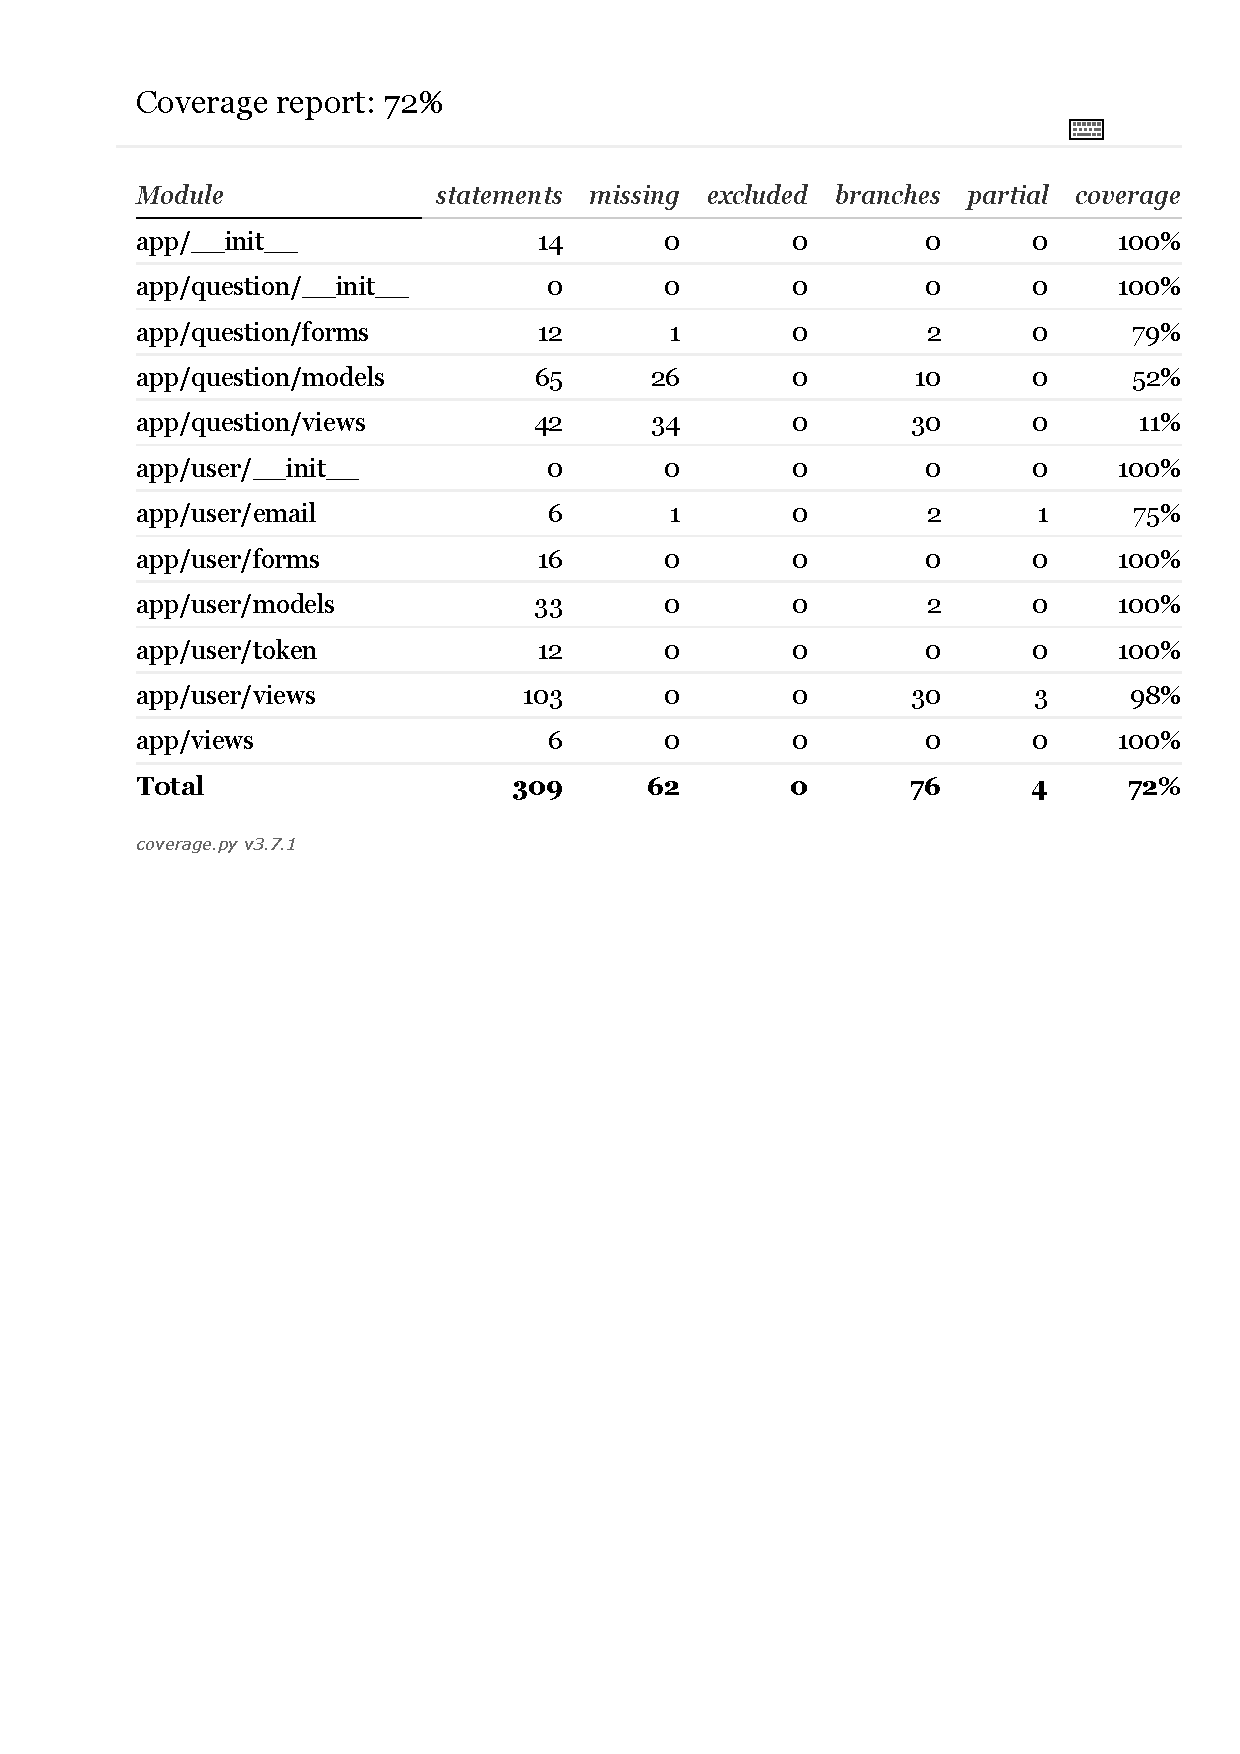
\includegraphics[width=0.8\linewidth]{figures/testcoverage.pdf}
    \caption{Oversigt over dækningsgraden af unittests. Det ses også hvor mange udtryk der er dækket af tests.}
    \label{fig:testcoverage}
\end{figure}

\begin{figure}[h]
    \centering
    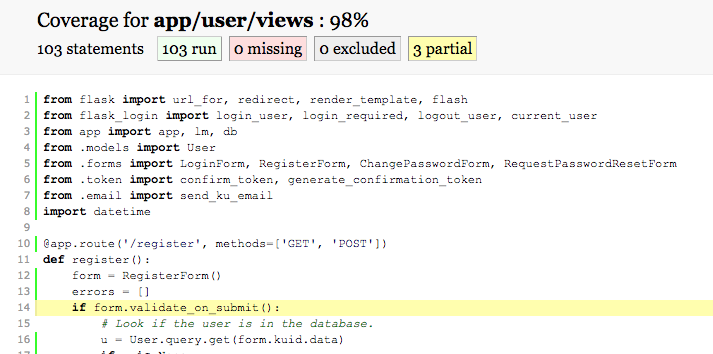
\includegraphics[width=0.8\linewidth]{figures/code_coverage.png}
    \caption{Eksempel på en grafik fremstilling, hvor et udtryk der kun delvist er dækket af tests fremhæves.}
    \label{fig:code_coverage}
\end{figure}

\section{Brugergrænseflade og interaktionsdesign}
\label{sec:brugergraenseflade}
\subsection{Screenshots}
I Appendix \ref{sec:screenshots} ses screenshots af brugergrænsefladen for de vigtigste dele af vores projekt. De optræder i en rækkefølge der illustrerer dynamikken i en studerendes interaktion med vores system. I toppen af de fleste screenshots ses en navigationsbar, hvor man bl.a. kan se hvem der er logget ind, man kan logge ud og man kan ændre sit password. Der er desuden i venstre side et slags logo hvor man kan trykke for at blive taget tilbage til forsiden.

På Figur \ref{fig:screenshot_login} ses et screenshot af den første del af vores brugergrænseflade en studerende vil møde, nemlig en login skærm. Hvis man allerede er registreret som bruger kan man her indtaste sig ku-id og sit valgte kodekord, og dermed logge på systemet. Hvis man ikke er oprettet som bruger er der et link der tager en videre til registrering. 

På Figur \ref{fig:screenshot_register} ses registrerings siden. Her kan man indtaste sig ku-id, vælge sig et kodeord og registrere sig. Systemet sender så en mail til den relevante ku-mail med et verificeringslink, og så snart den studerende har trykket på linket er vedkommende klar til at logge på systemet.

Når en studerende har logget sig ind i systemet vil han blive taget til index siden, som kan ses på Figur \ref{fig:screenshot_overview}. Her kan vedkommende få et overblik over de forskellige \emph{thresholds} og de dertil hørende \emph{subjects}. Den studerende kan så vælge hvilket emne han vil arbejde på og klikke på dets navn, hvilket fører ham videre til den næste del.

På Figur \ref{fig:screenshot_subject} ses \emph{subject} siden, hvor den studerende kan læse om det valgte emne, og hvis han finder det interessant, trykke på knappen og begynde at løse opgaver inden for det bestemte emne. De dummy-data vi har i databasen på nuværende tidspunkt er lidt simple, så derfor ser siden også lidt kedelig ud lige nu.

Når den studerende har trykket \emph{begin} vil han blive stillet en række opgaver, f.eks. multiple choice opgaver som den der kan ses på Figur \ref{fig:screenshot_question}. Den studerende kan så afgive sit svar, enten ved at indtaste et svar, afkryde de korrekte bokse eller trække svarmulighederne hen på de korrekte positioner, og trykke på \emph{answer} knappen. Der er desuden mulighed for at den studerende kan få hints til opgaven hvis det skulle være nødvendigt ved at trykke på den dertilhørende knap.

Når den studerende har svaret på en opgave vil vedkommende blive taget til svar-siden, som kan ses på Figur \ref{fig:screenshot_answer}. Her får den studerende feedback på sit svar, der kan variere fra en helt simpel besked i form af rigtigt eller forkert til et mere detaljeret svar der f.eks. kunne indeholde en relevant stack trace. På svar-siden er der desuden et såkaldt \emph{Learn-O-Meter}, hvor den studerende kan se hvor langt vedkommende er nået med at gennemføre det valgte emne.

Endeligt vil den studerende når vedkommende har gennemført et emne blive taget til en sidste side, som kan ses på Figur \ref{fig:screenshot_finish}, hvor der som det ser ud lige nu ikke står meget andet end \emph{Done}. Den studerende kan så trykke på \emph{finish} knappen, hvilket vil tage vedkommende til index siden, og derfra kan vedkommende så vælge et nyt emne at arbejde på eller logge ud.

\section{Projektsamarbejdet}
\label{sec:projektsamarbejdet}
Siden afleveringen af delrapport 1 har der været påskeferie, eksamensuge og blokferie, og vi er derfor ikke kommet så meget videre med projektet og har derfor heller ikke haft meget kontakt indbyrdes.

Her i blokferien har vi så haft vores andet møde med vores kunder, hvor vi snakkede om diverse aspekter af projektet og diskuterede opbygning og struktur af systemet. Vi er stadig på et stadie i vores diskussion med kunden hvor vi snakker relativt abstrakt om tingene, og vi er også som regel rimelig enige om tingen, og vi har derfor endnu ikke rigtig nået til at punkt hvor vi har følt at det var nødvendigt at tage et grundigt referat af hvad der blev snakket om.

Vi har desuden mødtes to gange i gruppen i blokferien, hvor vi har sat os i kantinen på DIKU for at sammen skrive delrapport 2, og det har fungeret udemærket. Vi har endnu ikke haft nogen deciderede \emph{møder} i gruppen hvor det har været nødvendigt med referat og dokumentation og den slags. Vi kommunikerer stadig på mail både internt i gruppen og med kunden, og vi bruger ligeledes Github til at dele vores arbejde med hinanden og med kunden, og begge dele fungerer også stadig udemærket.

Når vi har afleveret delrapport 2 er det planen at vi så vil mødes i gruppen og konkret diskuterer hvordan vi vil implementere vores system, f.eks. ift. opbygningen af databasen og hjemmesiden, og så sammen starte på at skrive koden. Når vi når dertil kan vi så se hvordan det går med arbejdet og med at dele det op imellem os og kommunikere indbyrdes, og der bliver det måske også mere relevant at dokumentere nogen af de ting vi snakker om i anden form end i delrapporterne.

\newpage
\appendix
\section{Versionsstyring}
\label{sec:versionsstyring}
Link til github: \url{https://github.com/christiankjaer/pop-webhelp}

\section{Changelog}
\label{sec:changelog}
\begin{tabular}{l l l}
08-04-2015 & CKL & Dokument oprettet. \\
14-04-2015 & CKL & Tilføjet use cases og krav. \\
16-04-2015 & LSE & Tilføjet UseCaseModel og BCE model. \\
16-04-2015 & CKL & Tilføjet review af Parnas og Clements. \\
17-04-2015 & TSH & Tilføjet review af Gould og Lewis. \\
17-04-2015 & LSE & Tilføjet Abstract og Projektsamarbejdet. \\
17-04-2015 & CKL & Tilføjet use cases, sekvensdiagram og klassediagram. \\
26-04-2015 & CKL & Tilføjet afsnit om tests. \\
30-04-2015 & CKL & Rettet til genaflevering og tilføjet systemdesign. \\
08-05-2015 & CKL & Tilføjet afsnit om strukturering. \\
10-05-2015 & LSE & Tilføjet Brugergrænseflade og screenshots, opdateret Systemdesign. \\
\end{tabular}

\section{Timeline}
\label{sec:timeline}
\begin{tabular}{l l p{8cm}}
11-03-2015 & Første møde med kunde: & Vi har første møde med kunden hvor vi snakker om hvad projektet går ud på og diskuterer krav og løsningsforslag. \\
16-04-2015 & Andet møde med kunde: & Vi har haft andet møde med kunden, hvor vi har snakket om modellen for de opgaver der skal være i systemet. \\
22-04-2015 & Internt møde i gruppen: & Vi har diskuteret databasemodeller, og vi er kommet frem til et databaseskema for denne iteration af systemet. Derudover fik vi udviklet i fællesskab på systemet. \\
27-04-2015 & Tredje møde med kunde: & Vi blev enige om en endelig funktionalitet for den første iteration af produktet. Derudover diskuterede vi udformingen af spørgmsålstyper og hvordan det hele skulle knyttes sammen. \\
07-05-2015 & Internt møde i gruppen: & Vi mødtes internt i gruppen for at diskutere udestående implementationsopgaver, og kigge på nogle ting sammen. \\
\end{tabular}

\bibliographystyle{alpha}
\bibliography{refs}{}

\section{ER-diagrammer}
\label{sec:er_diagrams}
\begin{figure}[h!]
    \centering
    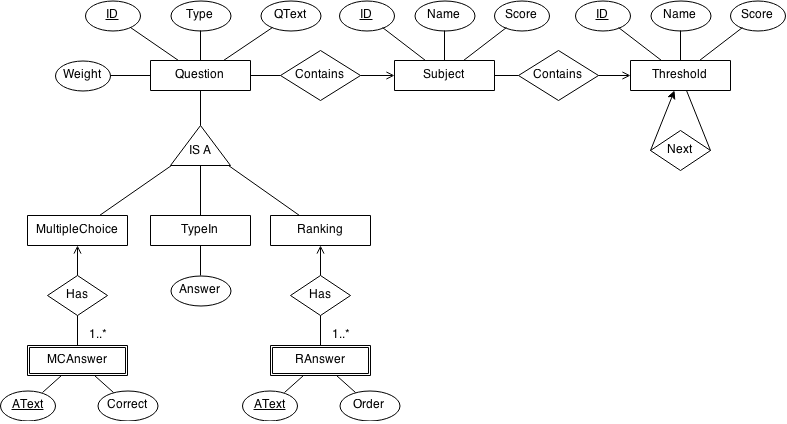
\includegraphics[width=0.8\linewidth]{figures/er_diagram/Qdb.png}
    \caption{ER-diagram over delen af databasen hvor spørgsmålene hører til.}
    \label{fig:er_diagram_question}
\end{figure}

\begin{figure}[h!]
    \centering
    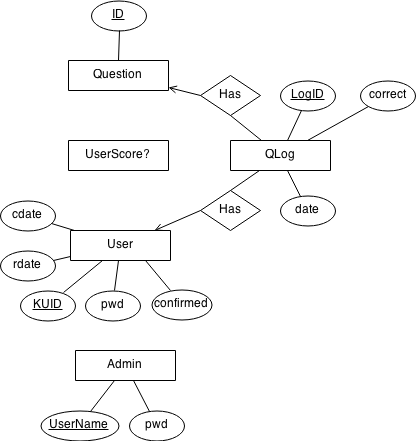
\includegraphics[width=0.8\linewidth]{figures/er_diagram/Logdb.png}
    \caption{ER-diagram over delen af databasen hvor loggen hører til.}
    \label{fig:er_diagram_log}
\end{figure}

\begin{figure}[h!]
    \centering
    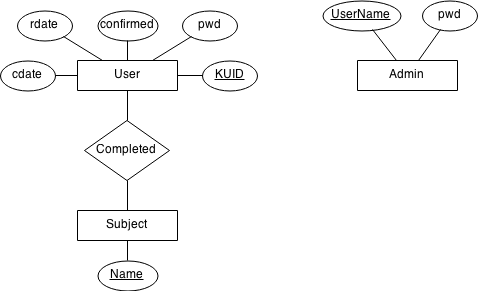
\includegraphics[width=0.8\linewidth]{figures/er_diagram/User.png}
    \caption{ER-diagram over delen af databasen hvor brugere og admins hører til.}
    \label{fig:er_diagram_user}
\end{figure}

\section{Brugergrænseflade screenshots}
\label{sec:screenshots}
\begin{figure}[h!]
    \centering
    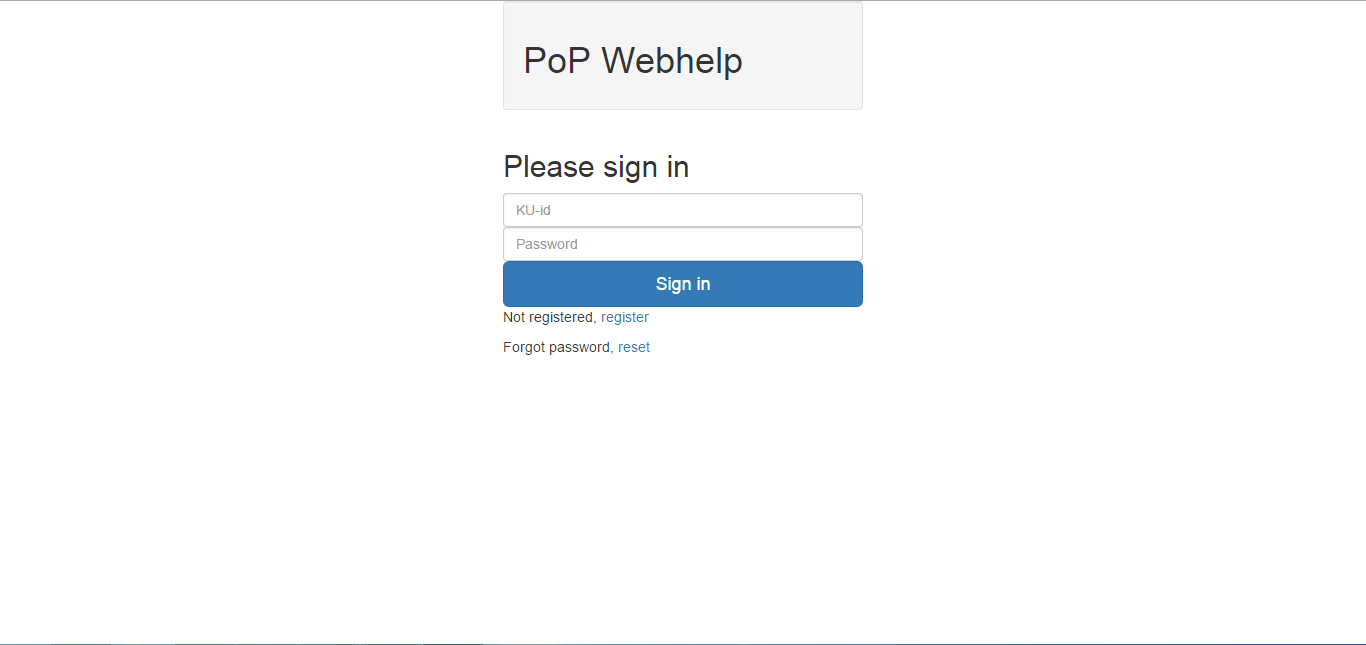
\includegraphics[width=1\linewidth]{figures/interface/login.png}
    \caption{Screenshot af login-siden.}
    \label{fig:screenshot_login}
\end{figure}


\begin{figure}[h!]
    \centering
    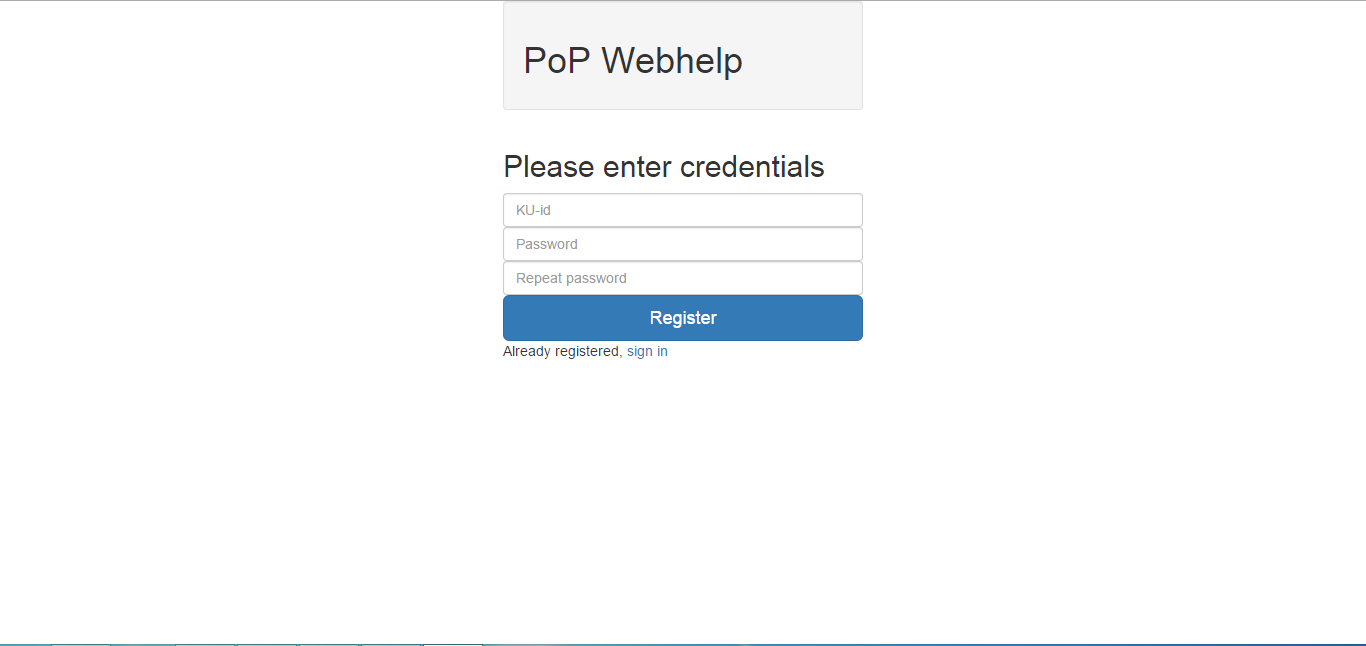
\includegraphics[width=1\linewidth]{figures/interface/register.png}
    \caption{Screenshot af registrerings-siden.}
    \label{fig:screenshot_register}
\end{figure}


\begin{figure}[h!]
    \centering
    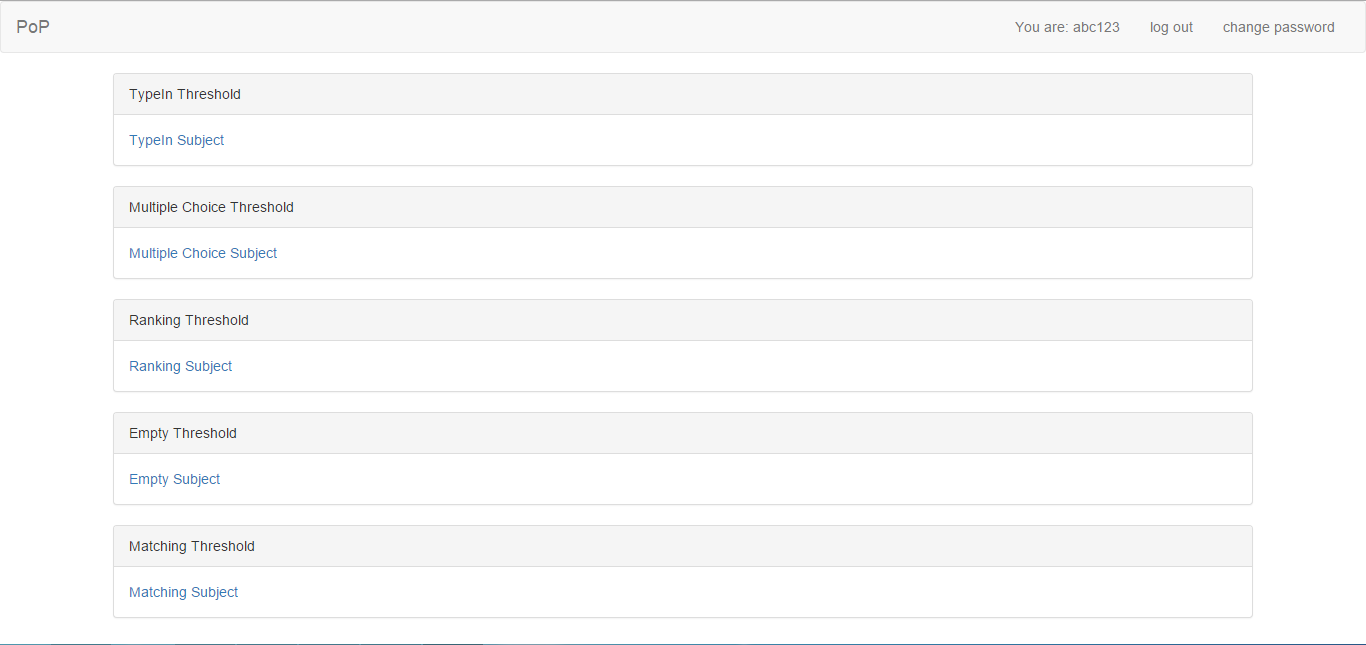
\includegraphics[width=1\linewidth]{figures/interface/overview.png}
    \caption{Screenshot af index-siden.}
    \label{fig:screenshot_overview}
\end{figure}


\begin{figure}[h!]
    \centering
    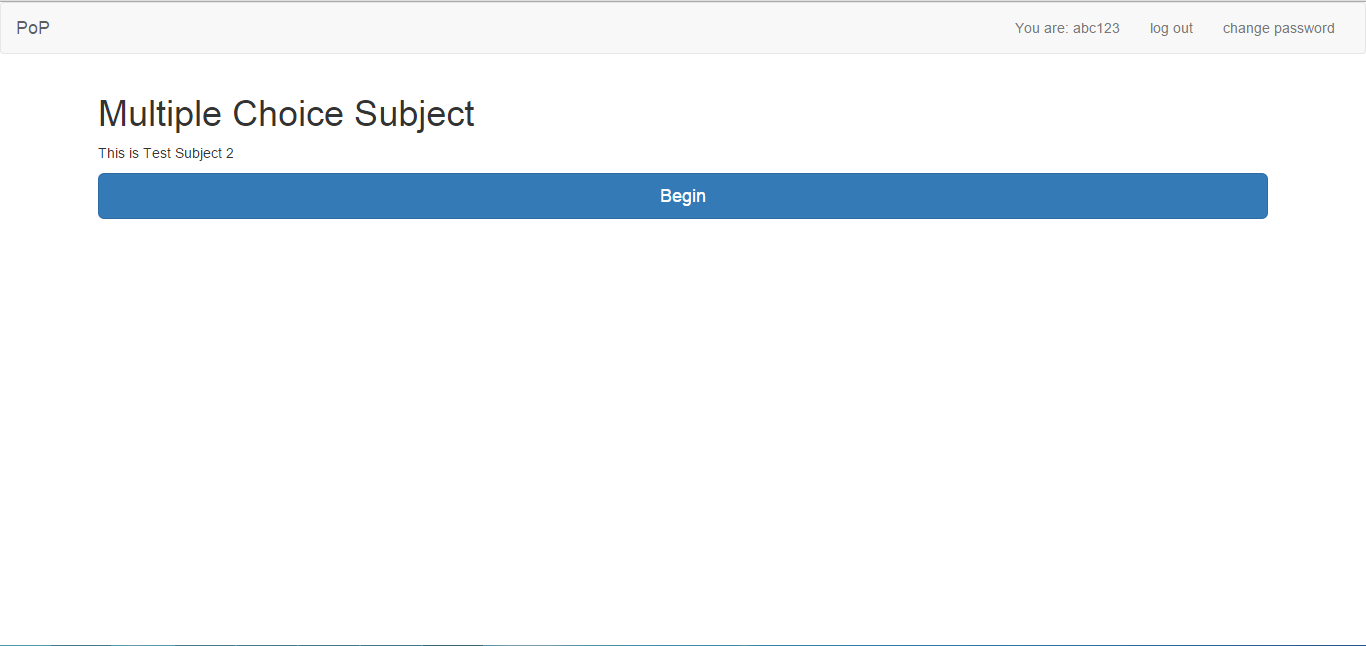
\includegraphics[width=1\linewidth]{figures/interface/subject.png}
    \caption{Screenshot af emne-siden.}
    \label{fig:screenshot_subject}
\end{figure}


\begin{figure}[h!]
    \centering
    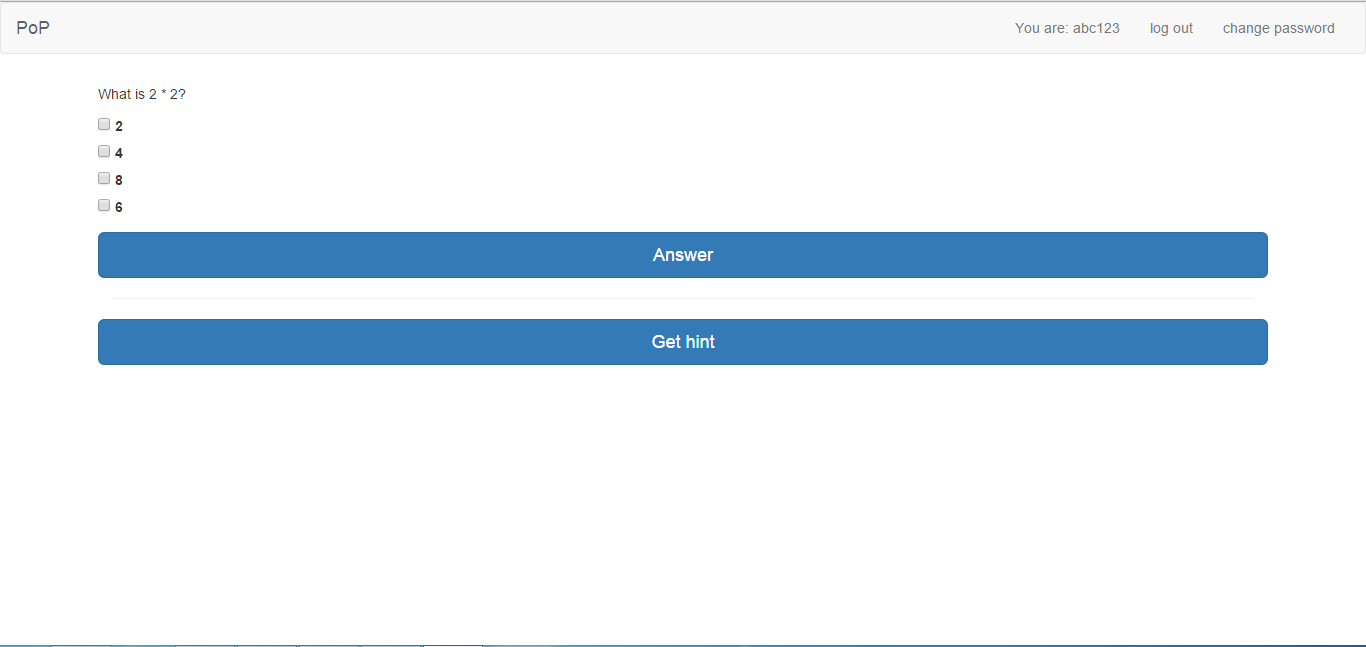
\includegraphics[width=1\linewidth]{figures/interface/question.png}
    \caption{Screenshot af spørgsmåls-siden.}
    \label{fig:screenshot_question}
\end{figure}


\begin{figure}[h!]
    \centering
    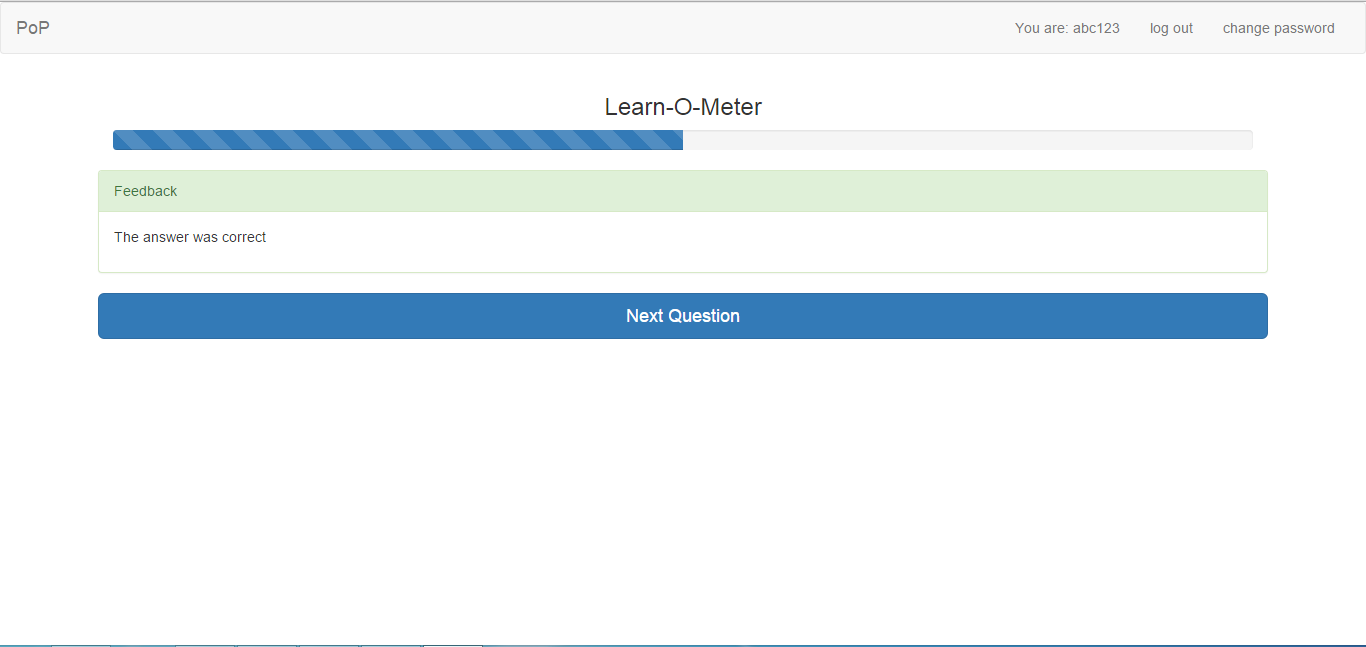
\includegraphics[width=1\linewidth]{figures/interface/answer.png}
    \caption{Screenshot af svar-siden.}
    \label{fig:screenshot_answer}
\end{figure}


\begin{figure}[h!]
    \centering
    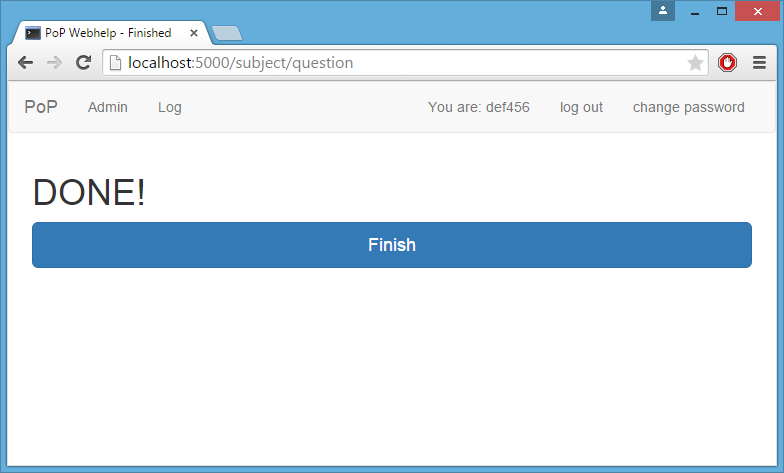
\includegraphics[width=1\linewidth]{figures/interface/finish.png}
    \caption{Screenshot af færdig-siden.}
    \label{fig:screenshot_finish}
\end{figure}

\end{document}
